% Copyright (C) 2008  Steve Chu.
% Permission is granted to use, modify, and redistribute under the terms
% of the Creative Commons 2.0 license.
% http://creativecommons.org/licenses/by-sa/2.0/

\documentclass{beamer}

%\usepackage{cctbase}

\usepackage{pgf,tikz}
\usepackage{url}
\usepackage{listings}
\usepackage{graphicx}

\def\cret{\tikz{
  \draw[->,rounded corners=2pt,thick,color=blue]
       (1.25ex,.75em) -- (1.25ex,0pt) -- (0pt,0pt);}}

\usetheme[secheader]{Madrid}
\lstset{language=sh}
\setbeamertemplate{navigation symbols}{}
\defbeamertemplate*{footline}{infolines theme without institution}
{
  \leavevmode%
  \hbox{%
  \begin{beamercolorbox}[wd=.333333\paperwidth,ht=2.25ex,dp=1ex,center]{author in head/foot}%
    \usebeamerfont{author in head/foot}\insertshortauthor
  \end{beamercolorbox}%
  \begin{beamercolorbox}[wd=.333333\paperwidth,ht=2.25ex,dp=1ex,center]{title in head/foot}%
    \usebeamerfont{title in head/foot}\insertshorttitle
  \end{beamercolorbox}%
  \begin{beamercolorbox}[wd=.333333\paperwidth,ht=2.25ex,dp=1ex,right]{date in head/foot}%
    \usebeamerfont{date in head/foot}\insertshortdate{}\hspace*{2em}
    \insertframenumber{} / \inserttotalframenumber\hspace*{2ex}
  \end{beamercolorbox}}%
  \vskip0pt%
}

\newcommand{\variable}[1]{{\color{violet}{\textsf{#1}}}}
\newcommand{\variablew}[1]{{{\textsf{#1}}}}
\newcommand{\filename}[1]{{\color{blue}{\textit{\begingroup \urlstyle{sf}\Url{#1}}}}}
\newcommand{\filenamew}[1]{{{\textit{\begingroup \urlstyle{sf}\Url{#1}}}}}
\newcommand{\command}[1]{`\texttt{#1}'}

% built files
\definecolor{bfile}{rgb}{.9,0.9,0.9}
% distributed generated files
\colorlet{dgfile}{yellow}
% auto* input file
\colorlet{afile}{green!33}
% tools
\definecolor{tfile}{rgb}{1.0,0.5,0.5}

\tikzstyle{afile}=[draw,fill=afile,shape=document,inner sep=1ex]
\tikzstyle{bfile}=[draw,fill=bfile,shape=document,inner sep=1ex]
\tikzstyle{dgfile}=[draw,fill=dgfile,shape=document,inner sep=1ex]
\tikzstyle{tfile}=[draw,fill=tfile,shape=rectangle,inner sep=1ex]

\newcommand\arr[1][]{\draw[thick,->,#1]}
\def\afile{\node[style=afile]}
\def\bfile{\node[style=bfile]}
\def\dgfile{\node[style=dgfile]}
\def\tfile{\node[style=tfile]}


\makeatletter

% Verbatim from the pgf manual:
\pgfdeclareshape{document}{
   \inheritsavedanchors[from=rectangle] % this is nearly a rectangle
   \inheritanchorborder[from=rectangle]
   \inheritanchor[from=rectangle]{center}
   \inheritanchor[from=rectangle]{north}
   \inheritanchor[from=rectangle]{south}
   \inheritanchor[from=rectangle]{west}
   \inheritanchor[from=rectangle]{east}
   % ... and possibly more
   \backgroundpath{% this is new
     % store lower right in xa/ya and upper right in xb/yb
     \southwest \pgf@xa=\pgf@x \pgf@ya=\pgf@y
     \northeast \pgf@xb=\pgf@x \pgf@yb=\pgf@y
     % compute corner of ``flipped page''
     \pgf@xc=\pgf@xb \advance\pgf@xc by-5pt % this should be a parameter
     \pgf@yc=\pgf@yb \advance\pgf@yc by-5pt
     % construct main path
     \pgfpathmoveto{\pgfpoint{\pgf@xa}{\pgf@ya}}
     \pgfpathlineto{\pgfpoint{\pgf@xa}{\pgf@yb}}
     \pgfpathlineto{\pgfpoint{\pgf@xc}{\pgf@yb}}
     \pgfpathlineto{\pgfpoint{\pgf@xb}{\pgf@yc}}
     \pgfpathlineto{\pgfpoint{\pgf@xb}{\pgf@ya}}
     \pgfpathclose
     % add little corner
     \pgfpathmoveto{\pgfpoint{\pgf@xc}{\pgf@yb}}
     \pgfpathlineto{\pgfpoint{\pgf@xc}{\pgf@yc}}
     \pgfpathlineto{\pgfpoint{\pgf@xb}{\pgf@yc}}
     \pgfpathlineto{\pgfpoint{\pgf@xc}{\pgf@yc}}
 }
}

\makeatother

% Adapted from texinfo.tex
\font\keyrm=cmtt8 scaled 1000
\font\keysy=cmsy9
\def\key#1{{\keyrm\textfont2=\keysy \leavevmode\hbox{%
  \raise0.4pt\hbox{$\langle$}\kern-.08em\vtop{%
    \vbox{\hrule\kern-0.4pt
     \hbox{\raise0.4pt\hbox{\vphantom{$\langle$}}#1}}%
    \kern-0.4pt\hrule}%
  \kern-.06em\raise0.4pt\hbox{$\rangle$}}}}

\newcommand{\mypart}[1]{\part{#1}\frame{\partpage \tableofcontents}}
\newcommand{\mysection}[1]{\section{#1}\frame{\frametitle{#1}\tableofcontents[sectionstyle=show/shaded,subsectionstyle=show/shaded/shaded]}}
\newcommand{\mysubsection}[1]{\subsection{#1}\frame{\frametitle{#1}\tableofcontents[sectionstyle=show/shaded,subsectionstyle=show/shaded/shaded]}}

%%%%%%%%%%%%%%%%%%%%%%%%%%%%%%%%%%%%%%%%%%%%%%%%%%%%%%%%%%%%%%%%%%%%%%
%%%%%%%%%%%%%%%%%%%%%%%%%%%%%%%%%%%%%%%%%%%%%%%%%%%%%%%%%%%%%%%%%%%%%%
%%%%%%%%%%%%%%%%%%%%%%%%%%%%%%%%%%%%%%%%%%%%%%%%%%%%%%%%%%%%%%%%%%%%%%

\begin{document}
%meta info
\title[Memcachedb: The Complete Guide]{Memcachedb: The Complete Guide}
\author[Steve Chu]{Steve Chu\\\url{stvchu@gmail.com}}
\institute{ICRD-Web@Sina}
\date{\today}
\subject{A complete introduction of Memcachedb}
\keywords{Memcachedb, memcache, BerkeleyDB}

%show cover
\begin{frame}
\titlepage
\end{frame}

\mypart{Getting Started}
\mysection{What is Memcachedb?}
\begin{frame}
\frametitle{What is Memcachedb?}
\begin{quote}
    "Memcachedb is a distributed key-value storage system designed for
    persistent."
\end{quote}

A complete memcached, but

\begin{itemize}
\item *NOT* a cache solution

Memcached is good enough for cache.

\item *NO* expiration

For memcache protocol compatible, still reserved, but we do nothing.

\item Totally for persistent

Transaction, replication, we do our best to achieve persistent.

\end{itemize}
\end{frame}

\mysection{Why Memcachedb?}
\begin{frame}
\frametitle{Why Memcachedb?(1/2)}

We have MySQL, we have PostgreSQL, we have a lot of RDBMSs, but why
we need Memcachedb?

\begin{itemize}
\item RDBMS is slow

All they have a complicated SQL engine on top of storage. 
Our data requires to be stored and retrieved damnable fast.

\item Not concurrent well

When thousands of clients, millions of requests happens... 

\item But the data we wanna store is very small size!

Cost is high if we use RDBMS.
\end{itemize}
\end{frame}

\begin{frame}
\frametitle{Why Memcachedb?(2/2)}

Many critical infrastructure services need fast, reliable data storage and retrieval,
but do not need the flexibility of dynamic SQL queries.
\begin{itemize}
\item Index, Counter, Flags
\item Identity Management(Account, Profile, User config info, Score)
\item Messaging
\item Personal domain name
\item meta data of distributed system
\item Other non-relatonal data
\item ...
\end{itemize}
\end{frame}

\mysection{Memcachedb Features}
\begin{frame}
\frametitle{Memcachedb Features}
\begin{itemize}
\item High performance read/write for a key-value based object

Rapid set/get for a key-value based object, not relational.
Benchmark will tell you the true later.

\item High reliable persistent storage with transaction

Transaction is used to make your data more reliable.

\item High availability data storage with replication

Replication rocks! Achieve your HA, spread your read, make your
transaction durable!

\item Memcache protocol compatibility

Lots of Memcached Client APIs can be used for Memcachedb, almost in any
language, Perl, C, Python, Java, ...

\end{itemize}
\end{frame}

\mysection{Supported Commands}
\begin{frame}
\frametitle{Standard Memcache Commands}
\begin{description}
\item[\command{get}]
  Retrieval of one or multiple items
\item[\command{set}]
  "Store this data"
\item[\command{add}]
  "Store this data, but only if the server *doesn't* already
  hold data for this key"
\item[\command{replace}]
  "Store this data, but only if the server *does*
  already hold data for this key"
\item[\command{delete}]
  deletes one item based a key
\item[\command{incr/decr}]
  Increment or decrement a numeric value. It's atomic!
\item[\command{stats}]
  shows the status of current deamon. 'stats', 'stats malloc', 'stats maps'
\end{description}
\end{frame}

\begin{frame}
\frametitle{Private Commands}
\begin{description}
\item[\command{db\_checkpoint}]
  does a checkpoint manuanlly.
\item[\command{db\_archive}]
  removes log files that are no longer needed.
\item[\command{stats bdb}]
  shows the status of BerkeleyDB.
\item[\command{rep\_ismaster}]
  shows whether the site is a master.
\item[\command{rep\_whoismaster}]
  shows which site is a master.
\item[\command{rep\_set\_priority}]
  sets the priority of a site for electing in replication.
\item[\command{rep\_set\_ack\_policy}]
  sets ACK policy of the replication.
\item[\command{rep\_set\_ack\_timeout}]
  sets ACK timeout value of the replication .
\item[\command{rep\_set\_bulk}]
  Enable bulk transfer or not in replication.
\item[\command{rep\_set\_request}]
  sets the minimum and maximum number of missing log records that a client waits before requesting retransmission.
\item[\command{stats rep}]
  shows the status of Replication.
\end{description}
\end{frame}

\mysection{Benchmark}
\begin{frame}
\frametitle{Environment}
\begin{itemize}
\item Box: Dell 2950III
\item OS: Linux CentOS 5
\item Version: memcachedb-1.0.0-beta
\item Client API: libmemcached
\end{itemize}
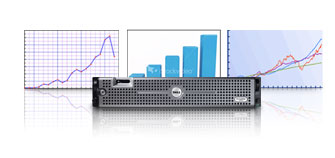
\includegraphics[height=3cm]{dell2950}
\end{frame}

\begin{frame}
\frametitle{Non-thread Version}
key: 16 value: 100B, 8 concurrents, every process does 2,000,000 set/get
\begin{block}{}
\texttt{memcachedb -d -r -u root -H /data1/mdbtest/ -N -v}
\end{block}
\begin{itemize}
\item Write
\begin{tabular}{l|c|c|c|c|c|c|c|c|c} \hline
No.      & 1   & 2   & 3   & 4   & 5   & 6   & 7   & 8   &  avg.\\ \hline
Cost(s)  & 807 & 835 & 840 & 853 & 859 & 857 & 865 & 868 &  848 \\ \hline
\end{tabular}
\begin{center}\textit{2000000 * 8 / 848 = 18868 w/s}\end{center}
\item Read
\begin{tabular}{l|c|c|c|c|c|c|c|c|c} \hline
No.      & 1   & 2   & 3   & 4   & 5   & 6   & 7   & 8   &  avg.\\ \hline
Cost(s)  & 354 & 354 & 359 & 358 & 357 & 364 & 363 & 365 &  360 \\ \hline
\end{tabular}
\begin{center}\textit{2000000 * 8 / 360 = 44444 r/s}\end{center}
\end{itemize}
\end{frame}

\begin{frame}
\frametitle{Thread Version}
key: 16 value: 100B, 8 concurrents, every process does 2,000,000 set/get
\begin{block}{}
\texttt{memcachedb -d -r -u root -H /data1/mdbtest/ -N -t 4 -v}
\end{block}
\begin{itemize}
\item Write
\begin{tabular}{l|c|c|c|c|c|c|c|c|c} \hline
No.      & 1   & 2   & 3   & 4   & 5   & 6   & 7   & 8   &  avg.\\ \hline
Cost(s)  & 663 & 669 & 680 & 680 & 684 & 683 & 687 & 686 &  679 \\ \hline
\end{tabular}
\begin{center}\textit{2000000 * 8 / 679 = 23564 w/s}\end{center}
\item Read
\begin{tabular}{l|c|c|c|c|c|c|c|c|c} \hline
No.      & 1   & 2   & 3   & 4   & 5   & 6   & 7   & 8   &  avg.\\ \hline
Cost(s)  & 245 & 249 & 250 & 248 & 248 & 249 & 251 & 250 &  249 \\ \hline
\end{tabular}
\begin{center}\textit{2000000 * 8 / 249 = 64257 r/s}\end{center}
\end{itemize}
\end{frame}

\mypart{MDB In Action}
\mysection{Installation}
\begin{frame}
\frametitle{Dependencies}
\begin{description}
\item[libevent]
  An event notification library that provides a mechanism to execute a callback function when a specific event occurs on a file descriptor or after a timeout has been reached. Now it supports /dev/poll, kqueue(2), event ports, select(2), poll(2) and epoll(4).

  \url{http://www.monkey.org/~provos/libevent/}

\item[BerkeleyDB]
  The industry-leading open source, embeddable database engine that provides developers with fast, reliable, local persistence with zero administration.

  \url{http://www.oracle.com/technology/products/berkeley-db/db/index.html}

\end{description}
\end{frame}

\begin{frame}[fragile]
\frametitle{Installing libevent}
\begin{block}{}
\begin{semiverbatim}
~ \% \alert<1>{\textit{tar zvxf libevent-1.3e.tar.gz}}
\uncover<2->{~ \% \alert<2>{\textit{cd libevent-1.3e}}}
\uncover<3->{~/libevent-1.3e \% \alert<3>{\textit{./configure}}
...}
\uncover<4->{~/libevent-1.3e \% \alert<4>{\textit{make}}
...}
\uncover<5->{~/libevent-1.3e \% \alert<5>{\textit{su}}
Password:}
\uncover<6->{/home/sc/libevent-1.3e # \alert<6>{\textit{make install}}
...}
\uncover<7->{/home/sc/libevent-1.3e # \alert<7>{\textit{exit}}}
\end{semiverbatim}
\end{block}
\end{frame}

\begin{frame}[fragile]
\frametitle{Installing BerkeleyDB}
\begin{block}{}
\begin{semiverbatim}
~ \% \alert<1>{\textit{tar zvxf db-4.6.21.tar.gz}}
\uncover<2->{~ \% \alert<2>{\textit{cd db-4.6.21}}}
\uncover<3->{~ \% \alert<3>{\textit{cd build\_unix}}}
\uncover<4->{~/db-4.6.21/build\_unix \% \alert<4>{\textit{../dist/configure}}
...}
\uncover<5->{~/db-4.6.21/build\_unix \% \alert<5>{\textit{make}}
...}
\uncover<6->{~/db-4.6.21/build\_unix \% \alert<6>{\textit{su}}
Password:}
\uncover<7->{/home/sc/db-4.6.21/build\_unix # \alert<7>{\textit{make install}}
...}
\uncover<8->{/home/sc/db-4.6.21/build\_unix # \alert<8>{\textit{exit}}}
\end{semiverbatim}
\end{block}
\end{frame}

\begin{frame}[fragile]
\frametitle{Installing Memcachedb}
\begin{block}{}
\begin{semiverbatim}
~ \% \alert<1>{\textit{tar zvxf memcachedb-1.0.3-beta.tar.gz}}
\uncover<2->{~ \% \alert<2>{\textit{cd memcachedb-1.0.3-beta}}}
\uncover<3->{~/memcachedb-1.0.3-beta \% \alert<3>{\textit{./configure }}#--enable-threads if
you wanna thread version
...}
\uncover<4->{~/memcachedb-1.0.3-beta \% \alert<4>{\textit{make}}
...}
\uncover<5->{~/memcachedb-1.0.3-beta \% \alert<5>{\textit{su}}
Password:}
\uncover<6->{/home/sc/memcachedb-1.0.3-beta # \alert<6>{\textit{make install}}
...}
\uncover<7->{/home/sc/memcachedb-1.0.3-beta # \alert<7>{\textit{exit}}}
\end{semiverbatim}
\end{block}
\end{frame}

\mysection{Running Options Explained}
\begin{frame}
\frametitle{Deamon Options}
\begin{description}
\item[\command{-p <num>}]
  TCP port number to listen on (default: 21201)
\item[\command{-l <ip\_addr>}]
  interface to listen on, default is INDRR\_ANY
\item[\command{-d}]
  run as a daemon
\item[\command{-r}]
  maximize core file limit
\item[\command{-u <username>}]
  assume identity of \texttt{<username>} (only when run as root)
\item[\command{-c <num>}]
  max simultaneous connections, default is 1024
\item[\command{-b <num>}]
  \alert{max item buffer size in bytes, default is 1KB}
\item[\command{-v}]
  verbose (print errors/warnings while in event loop)
\item[\command{-vv}]
  very verbose (also print client commands/reponses)
\item[\command{-P <file>}]
  save PID in \texttt{<file>}, only used with -d option
\end{description}
\end{frame}

\begin{frame}
\frametitle{BekerleyDB Options}
\begin{description}
\item[\command{-m <num>}]
  in-memmory cache size of BerkeleyDB in megabytes, default is 64MB
\item[\command{-f <file>}]
  filename of database, default is /data1/memcachedb/default.db
\item[\command{-H <dir>}]
  env home of database, default is /data1/memcachedb
\item[\command{-L <num>}]
  log buffer size in kbytes, default is 32KB
\item[\command{-C <num>}]
  do checkpoint every XX seconds, 0 for disable, default is 60s
\item[\command{-D <num>}]
  do deadlock detecting every XXX millisecond, 0 for disable, default is 100ms
\item[\command{-N}]
  \alert{enable DB\_TXN\_NOSYNC to gain big performance improved, default is off}
\end{description}
\end{frame}

\mysection{Managing Daemon}
\begin{frame}
\frametitle{Before start..}
Please take care this two options, a lot of mistakes have been made due to this:
\begin{description}
\item[\command{-b <num>}]
  \alert{max item buffer size in bytes, default is 1KB.}
  '-b option' determines MAX size of item can be stored. Just choose a suitable size.
   Following this formula: \\
   \textit{item\_buffer\_size(-b) = key\_size + data\_size + 37(Max)}

\item[\command{-N}]
  \alert{enable DB\_TXN\_NOSYNC to gain big performance improved, default is off.}
  By using '-N' option, 'ACID' in transaction will lose 'D'. The data in transaction
  log buffer may be gone when the machine loses power(So we need replication).
\end{description}

\end{frame}

\begin{frame}
\frametitle{How to start a deamon?}
Non-replication:
\begin{block}{}
\begin{semiverbatim}
 \textit{memcachedb -p21201 -d -r -u root -f 21201.db -H /data1/demo -N -P /data1/logs/21201.pid}
\end{semiverbatim}
\end{block}
\end{frame}

\begin{frame}
\frametitle{How to stop a deamon?}
Just kill it:
\begin{block}{}
\begin{semiverbatim}
 \textit{kill `cat /data1/logs/21201.pid`}
\end{semiverbatim}
\end{block}
When the deamon recives a signal of SIGTERM/SIGQUIT/SIGINT, it will do a checkpoint instantly and close the db and env resource normally. So don't be afraid, just kill it!
\end{frame}

\mysection{Commands Using telnet}
\begin{frame}[fragile]
\frametitle{set/get/delete a Item}
\begin{block}{}
\begin{semiverbatim}
~ \% \alert<1>{telnet 127.0.0.1 21201}
\uncover<2->{\alert<2>{Trying 127.0.0.1...
Connected to 127.0.0.1.
Escape character is '^]'.}}
\uncover<3->{\alert<3>{set test 0 0 4}}
\uncover<4->{\alert<4>{1234}}
\uncover<5->{\alert<5>{STORED}}
\uncover<6->{\alert<6>{get test}}
\uncover<7->{\alert<7>{VALUE test 0 4
1234
END}}
\uncover<8->{\alert<8>{delete test}}
\uncover<9->{\alert<9>{DELETED}}
\end{semiverbatim}
\end{block}
\end{frame}

\begin{frame}[fragile]
\frametitle{stats}
\begin{block}{}
\begin{semiverbatim}
~ \% \alert<1>{telnet 127.0.0.1 21201}
\uncover<2->{\alert<2>{Trying 127.0.0.1...
Connected to 127.0.0.1.
Escape character is '^]'.}}
\uncover<3->{\alert<3>{stats}}
\uncover<4->{\alert<4>{STAT pid 18547
STAT uptime 41385
STAT rusage\_user 0.084005
STAT rusage\_system 0.804050
STAT curr\_connections 1
...
STAT bytes\_read 5347
STAT bytes\_written 122797
STAT threads 1
END}}
\end{semiverbatim}
\end{block}
\end{frame}

\begin{frame}[fragile]
\frametitle{stats bdb}
\begin{block}{}
\begin{semiverbatim}
~ \% \alert<1>{telnet 127.0.0.1 21201}
\uncover<2->{\alert<2>{Trying 127.0.0.1...
Connected to 127.0.0.1.
Escape character is '^]'.}}
\uncover<3->{\alert<3>{stats bdb}}
\uncover<4->{\alert<4>{STAT cache\_size 67108864
STAT txn\_lg\_bsize 32768
STAT txn\_nosync 1
STAT dldetect\_val 100000
STAT chkpoint\_val 60
END}}
\end{semiverbatim}
\end{block}
\end{frame}

\mypart{Internals}
\mysection{The Big Picture}
\begin{frame}
\frametitle{Nonthread Version}
\begin{center}
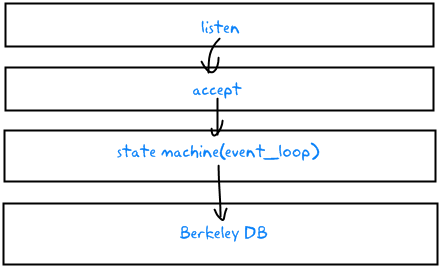
\includegraphics[scale=1,width=0.70\textwidth]{mdb_nonthread.png}
\end{center}
\end{frame}
\begin{frame}
\frametitle{Thread Version}
\begin{center}
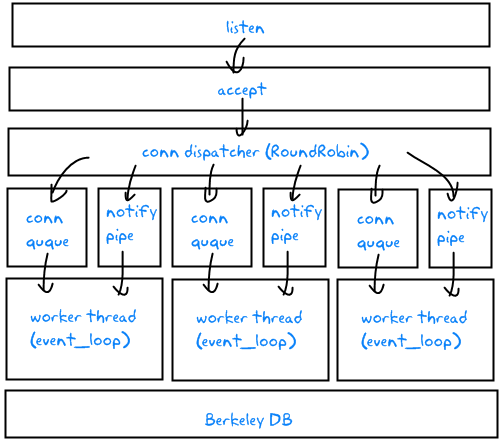
\includegraphics[scale=1,width=0.70\textwidth]{mdb_thread.png}
\end{center}
\end{frame}
\begin{frame}
\frametitle{The Backend: BerkeleyDB}
\url{http://www.oracle.com/technology/products/berkeley-db/db/index.html}
\begin{center}
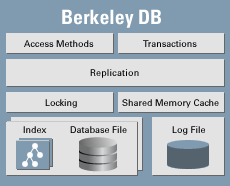
\includegraphics[scale=1,width=0.50\textwidth]{berkeley-db-stack.png}
\end{center}
\end{frame}

\mypart{Replication}
\mysection{Overview}
\begin{frame}
\frametitle{Replication Model}
Consistency is an important issue that every engineer must resolve when designing a distributed system. The BerkeleyDB replication framework resolves this by following a \texttt{single master, multiple replica} model. 
\begin{center}
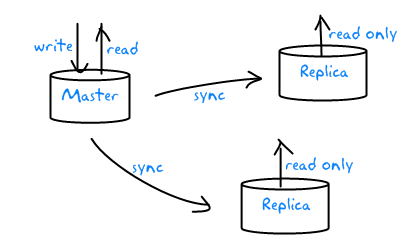
\includegraphics[scale=1,width=0.70\textwidth]{replication.png}
\end{center}
\end{frame}

\begin{frame}
\frametitle{Replication Benefits}
\begin{itemize}
\item Improve application reliability \\
By spreading your data across multiple machines, you can ensure that your application's data continues to be available even in the event of a hardware failure on any given machine in the replication group.  
\item Improve read performance \\
By using replication you can spread data reads across multiple machines on your network. 
\item Improve transactional commit performance and data durability guarantee\\
Replication allows you to avoid this disk I/O and still maintain a degree of durability by \texttt{committing to the network}. So we can use '-N' option for better performance but never lose durability(The D of ACID).
\end{itemize}
\end{frame}

\mysection{Replication Patterns}
\begin{frame}
\frametitle{ACK Policy(1/2)}
Messaging is the key facility that implements replication. 
How to process a message influences your data reliability and performance. 
Now we go deep into these policies:
\begin{description}
\item[\command{DB\_REPMGR\_ACKS\_ALL}]
The master should wait until all replication clients have acknowledged each permanent replication message. 
\item[\command{DB\_REPMGR\_ACKS\_ALL\_PEERS}]
The master should wait until all electable peers have acknowledged each permanent replication message (where "electable peer" means a client capable of being subsequently elected master of the replication group). 
\item[\command{DB\_REPMGR\_ACKS\_NONE}]
The master should not wait for any client replication message acknowledgments. 
\item[\command{DB\_REPMGR\_ACKS\_ONE}]
The master should wait until at least one client site has acknowledged each permanent replication message. 
\end{description}
\end{frame}

\begin{frame}
\frametitle{ACK Policy(2/2)}
\begin{description}
\item[\command{DB\_REPMGR\_ACKS\_ONE\_PEER}]
The master should wait until at least one electable peer has acknowledged each permanent replication message (where "electable peer" means a client capable of being subsequently elected master of the replication group). 
\item[\command{DB\_REPMGR\_ACKS\_QUORUM}]
    The master should wait until it has received acknowledgements from the minimum number of electable peers sufficient to ensure that the effect of the permanent record remains durable if an election is held (where "electable peer" means a client capable of being subsequently elected master of the replication group). This is the default acknowledgement policy. 
\end{description}
\alert{Note:} The current implementation requires all sites in a replication group configure the same acknowledgement policy.
\end{frame}

\begin{frame}
\frametitle{Performance vs Data Reliability}
\begin{description}
\item[\command{ACK\_ALL}]
More data reliability, but poor performance due to the blocked thread waiting for ack(the thread can not continue to write).
\item[\command{ACK\_NONE}]
Better performance, but may cause reliable problem because of the unstable network between a master and replica(the data of repllica may be out-of-date).  
\end{description}
So we must do a tradeoff:\\
Let Replica who in the same LAN with Master do the reliable thing, 
and let the site far from the Master recieves replication message with ACK\_NONE. 
\end{frame}

\begin{frame}
\frametitle{How ACK\_NONE Replicas catch up with Master}
\begin{itemize}
\item Restart your replica daemon, and force a replica sync with master.\\
Not that flexible..
\item Set a minor number of missing log records that a client waits before requesting retransmission.\\
A replication client checks the log sequence number of each incoming log record, and can detect gaps in the sequence. If some log records are lost due to network problems, then when later log records arrive the client detects the missing records. The client waits for some number of out-of-sequence log records before issuing the request for retransmission. 
\end{itemize}
\end{frame}

\begin{frame}
\frametitle{Replication over LAN}
\begin{center}
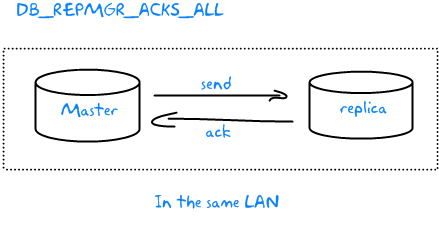
\includegraphics[scale=1,width=0.70\textwidth]{rep_lan.png}
\end{center}
\end{frame}

\begin{frame}
\frametitle{Replication over WAN}
\begin{center}
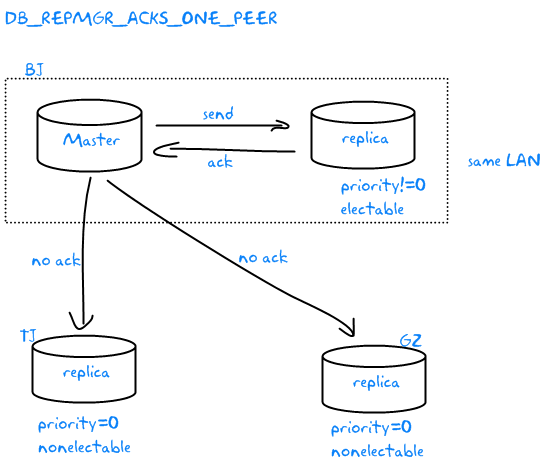
\includegraphics[scale=1,width=0.70\textwidth]{rep_wan.png}
\end{center}
\end{frame}

\mysection{Replication Howto}
\begin{frame}
\frametitle{Design your deployment}
Your deployment based the replication pattern you choose, and try to think about these:
\begin{itemize}
\item Network QoS
\item How large your dataset
\item Proportion of read/write
\item Throughput of read/write
\item The replication group size
\item ...
\end{itemize}
Find out:
\begin{itemize}
\item How many sites? Over LAN or WAN?
\item Which ACK policy to take?
\item Which is electable or not?
\item ...
\end{itemize}

\end{frame}

\begin{frame}
\frametitle{Prepare your dataset}
If your initial dataset is empty, then go to next step.. otherwise follow this:
\begin{itemize}
\item Initialize your data into a Master site.
\item Do a hotbackup of your master environment and compress all data into a package.
\item Drag the package to where replica locates, decompress, and go to next step.
\end{itemize}
\begin{center}
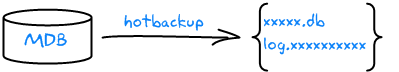
\includegraphics[scale=1,width=0.70\textwidth]{hotbackup.png}
\end{center}
\end{frame}
\begin{frame}
\frametitle{Start and Configure the Daemon(1/4)}
Replication Options:
\begin{description}
\item[\command{-R}]
  identifies the host and port used by this site (required).
\item[\command{-O}]
  identifies another site participating in this replication group
\item[\command{-M/-S}]
  start as a master or slave
\end{description}
Start as a master:
\begin{block}{}
\begin{semiverbatim}
 \textit{memcachedb -p21201 -d -r -u root -f 21201.db -H /data1/demo -N -P /data1/logs/21201.pid -R 127.0.0.1:31201 -M}
\end{semiverbatim}
\end{block}
Start as a slave:
\begin{block}{}
\begin{semiverbatim}
 \textit{memcachedb -p21202 -d -r -u root -f 21202.db -H /data1/demo -N -P /data1/logs/21202.pid -R 127.0.0.1:31202 -O 127.0.0.1:31201 -S}
\end{semiverbatim}
\end{block}
\end{frame}

\begin{frame}
\frametitle{Start and Configure the Daemon(2/4)}
Besides running replication options, there are private commands available to configure the current site:
\begin{description}
\item[\command{stats rep}]
  shows the status of Replication.
\item[\command{rep\_set\_priority}]
  sets the priority of a site for electing in replication.
\item[\command{rep\_set\_request}]
  sets the minimum and maximum number of missing log records that a client waits before requesting retransmission.
\item[\command{rep\_set\_bulk}]
  Enable bulk transfer or not in replication.
\item[\command{rep\_set\_ack\_timeout}]
  sets ACK timeout value of the replication .
\item[\command{rep\_set\_ack\_policy}]
  sets ACK policy of the replication.
\begin{center}
\begin{tabular}{lcr}
DB\_REPMGR\_ACKS\_ALL           &     1 \\
DB\_REPMGR\_ACKS\_ALL\_PEERS    &     2 \\
DB\_REPMGR\_ACKS\_NONE          &     3 \\
DB\_REPMGR\_ACKS\_ONE           &     4 \\
DB\_REPMGR\_ACKS\_ONE\_PEER     &     5 \\
DB\_REPMGR\_ACKS\_QUORUM        &     6 \\
\end{tabular}
\end{center}
\end{description}
\end{frame}

\begin{frame}[fragile]
\frametitle{Start and Configure the Daemon(3/4)}
\begin{block}{}
\begin{semiverbatim}
~ \% \alert<1>{telnet 127.0.0.1 21202}
\uncover<2->{\alert<2>{Trying 127.0.0.1...
Connected to 127.0.0.1.
Escape character is '^]'.}}
\uncover<3->{\alert<3>{rep\_set\_priority 0}}
\uncover<4->{\alert<4>{0}}
\uncover<5->{\alert<5>{rep\_set\_ack\_policy 5}}
\uncover<6->{\alert<6>{5}}
\uncover<7->{\alert<7>{rep\_set\_ack\_timeout 50000}}
\uncover<8->{\alert<8>{50000}}
\uncover<9->{\alert<9>{rep\_set\_request 2 4}}
\uncover<10->{\alert<10>{2/4}}
\end{semiverbatim}
\end{block}
\end{frame}

\begin{frame}[fragile]
\frametitle{Start and Configure the Daemon(4/4)}
\begin{block}{}
\begin{semiverbatim}
~ \% \alert<1>{telnet 127.0.0.1 21202}
\uncover<2->{\alert<2>{Trying 127.0.0.1...
Connected to 127.0.0.1.
Escape character is '^]'.}}
\uncover<3->{\alert<3>{stats rep}}
\uncover<4->{\alert<4>{STAT rep\_whoismaster 127.0.0.1:31201
STAT rep\_localhp 127.0.0.1:31202
STAT rep\_ismaster REP\_FALSE
STAT rep\_priority 0
STAT rep\_ack\_policy 5
STAT rep\_ack\_timeout 50000
STAT rep\_bulk 1
STAT rep\_request 2/4
STAT rep\_next\_lsn 25/6752622
END
}}
\end{semiverbatim}
\end{block}
\end{frame}

\mypart{Managing and Monitoring}
\mysection{Managing DB Files}

\begin{frame}
\frametitle{Home Environment}
\begin{quote}In order to transaction protect your database operations, you must use an environment. \end{quote}
\begin{quote}An environment, represents an encapsulation of one or more databases and any associated log and region files. \end{quote}
There are three types of files in a environment:
\begin{description}
\item[\command{Database files}]
  the exact files that store your data.
\item[\command{Log files}]
  all your transcations you commit first come into logs.
\item[\command{Region files}]
  files that back the share memory region using mmap().
\end{description}
\end{frame}

\begin{frame}
\frametitle{Checkpoint(1/2)}
\begin{itemize}
\item When databases are modified (that is, a transaction is committed), the modifications are recorded in DB's logs
\item But the increased logs make recovery take too long time.
\item Log files also have more unnecessary data than database file.
\item Log files make catastrophic recovery possible.
\end{itemize}

So here comes Checkpoint:
\begin{center}

\includegraphics[scale=1,width=0.70\textwidth]{checkpoint.png}
\end{center}
\end{frame}

\begin{frame}
\frametitle{Checkpoint(2/2)}
The checkpoint:
\begin{itemize}
\item Flushes dirty pages from the in-memory cache.
\item Writes a checkpoint record.
\item Flushes the log.
\item Writes a list of open databases.
\end{itemize}
How to do checkpoint in Memcachedb:
\begin{itemize}
\item Run checkpoint periodically with '-C' option
\item The private command: 'db\_checkpoint'
\end{itemize}

\end{frame}

\begin{frame}
\frametitle{Backup Procedures}
\textbf{Hot Backup}
\begin{block}{}
\begin{semiverbatim}
 \textit{/usr/local/BerkeleyDB.4.6/bin/db\_hotbackup [-c] -h home -b backup\_dir}
\end{semiverbatim}
\end{block}
DB files has a high compression ratio, and use \textit{gzip} and \textit{tar} to archive.
\end{frame}

\begin{frame}
\frametitle{Recovery Procedures}
\begin{itemize}
\item Normal Recovery

Put database files and log files since the last checkpoint(or a hotbackup copy) into a empty home environemt,
Start the deamon on this environment, the deamon will do recovery automatically. Also it can be done by using 
standalone utility 'db\_recover':
\begin{block}{}
\begin{semiverbatim}
 \textit{/usr/local/BerkeleyDB.4.6/bin/db\_recover -f -h home}
\end{semiverbatim}
\end{block}

\item Catastrophic Recovery

Put all your database files and all log files(since environment created) into a empty home environment, Use standalone utility 'db\_recover' with option '-c':
\begin{block}{}
\begin{semiverbatim}
 \textit{/usr/local/BerkeleyDB.4.6/bin/db\_recover -cf -h home}
\end{semiverbatim}
\end{block}
\end{itemize}
\end{frame}

\begin{frame}
\frametitle{Removing Log Files}
Log Files in which transactions have been checkpointed into database file can be removed directly or archived to offline storage devices. You can remove this log files by 
\begin{itemize}
\item using private command: 'db\_archive' 
\item using standalone utility 'db\_archive' with option '-d':
\begin{block}{}
\begin{semiverbatim}
 \textit{/usr/local/BerkeleyDB.4.6/bin/db\_archive -d -h home}
\end{semiverbatim}
\end{block}
\end{itemize}
\alert{Warning:} log file removal is likely to make catastrophic recovery impossible. If the data is very important(I mean if the data is lost, you are over.), you'd better archive them to offline storage devices instead of removal.
\end{frame}

\mysection{Monitoring}
\begin{frame}
\frametitle{Overview}
There are four ways now available for monitoring Memcachedb:
\begin{itemize}
\item the raw 'stats' commands: 'stats', 'stats bdb', 'stats rep'
\item the standalone utility 'db\_stat'
\item the coming along monitoring tool 'tools/mdbtop.py'
\item writing your own monitoring tool using 'tools/memcache.py'
\end{itemize}
\end{frame}

\begin{frame}
\frametitle{'stats' command}
There are a few of 'stats' commands in Memcachedb:
\begin{description}
\item[\command{stats}]
shows the status of current deamon.
\item[\command{stats bdb}]
shows the status of BerkeleyDB.
\item[\command{stats rep}]
shows the status of Replication.
\end{description}

Just telnet in, and use them. Some of Memcached Client APIs support 'stats' command, but some not. 
If you find no one can do it, have a try of patched 'memcache.py' in 'tools/' of distribution.
\end{frame}

\begin{frame}
\frametitle{db\_stat}
BerkeleyDB distribution has a standalone utility 'db\_stat' that can help us
 to get statistics for Berkeley DB environments.
\begin{description}
\item[\command{-c}]
Display locking subsystem statistics
\item[\command{-l}]
Display logging subsystem statistics
\item[\command{-m}]
Display cache statistics
\item[\command{-r}]
Display replication statistics
\item[\command{-t}]
Display transaction subsystem statistics\\
...
\end{description}
See 'docs/utility/db\_stat.html' in BerkeleyDB distribution for more info.\\
\alert{Warning:} '-d' option which displays database statistics for the specified file will be very expensive(that requires traversing the database), do not use it on a high traffic Memcachedb daemon.
\end{frame}

\begin{frame}[fragile]
\frametitle{mdbtop.py}
'mdbtop.py' is a monitoring tool coming along with distribution. 
It is built on the patched 'memcache.py' Python API. 
\begin{block}{}
\begin{semiverbatim}
 \textit{./mdbtop.py <mdbtop.cfg> [rep]}
\end{semiverbatim}
\end{block}
'mdbtop.cfg' is the configure file that mdbtop.py uses:
\begin{block}{\filenamew{mdbtop.cfg}}
\begin{lstlisting}[language=Python]
[Server]
server1 = 127.0.0.1:21201
server2 = 127.0.0.1:21202
[View]
interval = 1
\end{lstlisting}
\end{block}

[rep] option is for only replication syncing monitoring.
\end{frame}

\begin{frame}[fragile]
\frametitle{memcache.py}
The patched 'memcache.py' now has all private commands supported and
 you can write your own monitoring tools depending on these APIs:
\begin{block}{\filenamew{memcache.py}}
\begin{lstlisting}[language=Python]
import memcache
mc = memcache.Client(['127.0.0.1:21202'], debug=0)
mc.db_archive()
mc.db_checkpoint()
mc.rep_ismaster()
mc.rep_whoismaster()
mc.rep_set_priority(100)
mc.rep_set_ack_policy(5)
mc.rep_set_ack_timeout(20000)
mc.rep_set_request(4, 16)
mc.disconnect_all()
\end{lstlisting}
\end{block}
\end{frame}

\mypart{The End}
\begin{frame}
\frametitle{Project info}
Homepage: \url{http://memcachedb.org}

Mailing list: \url{http://groups.google.com/group/memcachedb}
\begin{itemize}
\item To subscribe to maillist, send email to memcachedb-subscribe@googlegroups.com
\item To post to maillist, send email to memcachedb@googlegroups.com
\item To unsubscribe from maillist, send email to memcachedb-unsubscribe@googlegroups.com 
\end{itemize}

Please report your bugs and issues to the Maillist. 
\end{frame}

\begin{frame}
\frametitle{Q/A}
\begin{center}
Any question?
\end{center}
\end{frame}

\end{document}
